\section{Sistematika Dokumen}
Dalam format latex memiliki kemampuan untuk membuat suatu susunan yang struktural atau tertata dengan rapi
seperti \textit{bab,subbab,} dan sebagainya.

\begin{table}[h]
\caption{Small Table}
\centering

\begin{tabular}{|c|c|}
\hline
\textbf{Struktur}&\textbf{penulisan}\\
\hline
Bagian&{part}\\
\hline
Bab&{chapter}\\
\hline
subbab&{section}\\
\hline
subsubbab&subsection\\
\hline
subsubsubbab&subsubsection\\
\hline
parangraf berjudul&{parangraph}\\
\hline
anak parangraf berjudul &{subparangraph}\\
\hline
\end{tabular}

\label{table:contoh}
\end{table}
 
\section{Alignment}
Alignment adalah perataan baris pada LateX. terdapat 3 jenis pada perataan tersebut yaitu rata kiri,rata kanan atau rata tengah. pada dokumen LateX memiliki perataan yang secara default sudah diatur dan memiliki perataan justified atau biasa disebut rata kanan.
Misalkan saat ini kita ingin melakukan pengaturan dokumen rata kiri, maka perintah yang dimasukan yaitu :
\lstinputlisting[caption=Contoh Perintah Membuat Rata Kiri,label={lst:perataan}]{src/1/aligmentkiri.tex}
atau bisa juga kira masukan perintah yang sama untuk rata kiri.
\lstinputlisting[caption=Contoh Perintah Membuat Rata Kanan,label={lst:perataan}]{src/2/aligmentkanan.tex}

\section{Document class}

Pada dokumen Latex terdapat atau mempunyai beberapa struktur yang dicirikan dengan blok yang diberi apit oleh perintah begin dan end. Latex memberikan pilihan Class dokuman yang bisa di pakai, antara lain aadlah Book, Report, Article dan lain sebagainya. Class document book merupakan Class Document yang paling tepat untuk menulis, karena dapat mendukung table of contents yang dapat berfungsi langsung untuk generate daftar isi secara langsung.


Format ukuran font pada latex \ref{labelgambar1}

\begin{figure}[ht]
\centerline{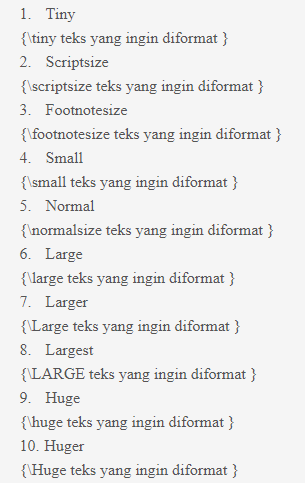
\includegraphics[width=0.7\textwidth]{figures/1class.PNG}}
\caption{ukuran font}
\label{labelgambar1}
\end{figure}

Dalam memberikan penulisan judul pada format latex biasanya di letakkan pada awal document, untuk cara penulisan nya dapat dilakukan sebagai berikut:
\begin{enumerate}
  \item \textit{backslash} document class kurung kurawal a4papper, ukuran yang di inginkan tutup kurawal lalu report
  \item \textit{backslash} begin buka kurawal document tutup kurawal
  \item \textit{backslash} begin buka kurawal judul document tutup kurawal
  \item \textit{backslash} autor buka kurawal nama penulis tutup kurawal
  \item \textit{backslash} date buka kurawal tanggal pembuatan tutup kurawal
  \item \textit{backslash} maketitle
  \item \textit{backslash} and buka kurawal document tutup kurawal
\end{enumerate}

\section{Costum Command}
Sesuai  dengan  namanya Costum Command, dimana ke unggulan latex ada fitur yang satu ini, Pembuat dokumen ini dapat  membuat macro untuk kebutuhan yang sifatnya spesifik dan berulang-ulang, dimana costum cummad dapat melakukan tanda bintang berjejer sebagai penanda garis. Pada Pengaturan huruf lateks dibuat dengan menggunakan tag atau perintah khusus yang menyediakan beberapa cara untuk memformat dokumen Anda. Kadang-kadang perintah standar tidak cukup untuk memenuhi beberapa kebutuhan spesifik.
